


\newsavebox{\detectextrema}
\begin{lrbox}{\detectextrema} 
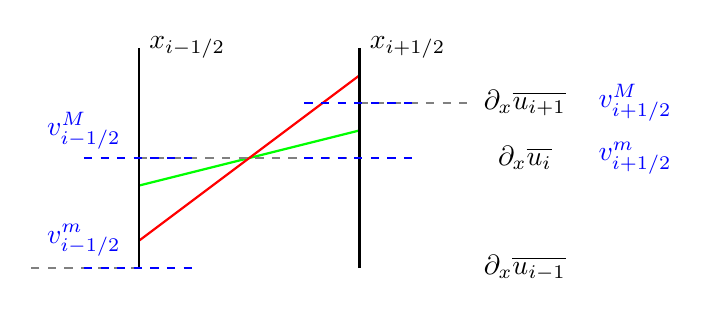
\begin{tikzpicture}[scale=0.7]
\draw[green, thick] (-2,-1/2) -- (2,1/2);
\draw[red,   thick] (-2,-3/2) -- (2,3/2);
\draw[black, thick] (-2,-4/2) -- (-2,4/2) node[right] {$x_{i-1/2}$};
\draw[black, thick] ( 2,-4/2) -- ( 2,4/2) node[right] {$x_{i+1/2}$};
\draw[gray,  thick,dashed] (-2, 0/2) -- (2,0/2);
\draw[gray,  thick,dashed] (-2, -4/2) -- (-4,-4/2);
\draw[gray,  thick,dashed] (2, 2/2)  -- ( 4,2/2);

\draw[blue,  thick,dashed] (-3,-4/2)  -- (-1,-4/2);
\draw[blue,  thick,dashed] (-3, 0/2)  -- (-1, 0/2);

\draw[blue,  thick,dashed] (1, 0/2)  -- ( 3,0/2);
\draw[blue,  thick,dashed] (1, 2/2)  -- ( 3,2/2);

\coordinate (s1) at (5,0) ;\coordinate (s2) at (5,1) ;\coordinate (s3) at (5,-2);
\coordinate (s4) at (7,0) ;\coordinate (s5) at (7,1) ;
\coordinate (s6) at (-3,0.5) ;\coordinate (s7) at (-3,-1.5) ;
\node at (s1) {$\partial_x \overline{u_i}$};
\node at (s2) {$\partial_x \overline{u_{i+1}}$};
\node at (s3) {$\partial_x \overline{u_{i-1}}$};

\node[blue] at (s4) {$v_{i+1/2}^m$};\node[blue] at (s5) {$v_{i+1/2}^M$};
\node[blue] at (s7) {$v_{i-1/2}^m$};\node[blue] at (s6) {$v_{i-1/2}^M$};
\end{tikzpicture}
\end{lrbox} 
